% Preamble
\documentclass[xcolor=table,handout]{beamer}

% Title/Author/Date
\title{Introduction to Robotframework}  
\author[K. Bellock]{Kenneth Bellock}
\titlegraphic{%
    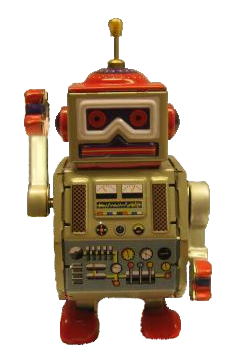
\includegraphics[height=.37\textheight]{robot-wave}

    \tiny \url{http://robotframework.org}
}
\date{\vspace*{-2.5em}\par \today} 

% Package Dependencies
\usepackage{beamerthemeshadow}
\usepackage{color}
\usepackage{colortbl}
\usepackage{booktabs}
\usepackage{adjustbox}
\usepackage{lmodern}
\usepackage{tikz}
\usepackage{pgfpages}
\usepackage{pgfgantt}
\usepackage{pgfcalendar}
\usepackage{pgfplots}
\pgfplotsset{compat=newest}
\usepackage{calc}
\usepackage{ifthen}
\usepackage{tcolorbox}
\usepackage[edges]{forest}
\tcbuselibrary{theorems,listings,skins,breakable,minted}
\usetikzlibrary{shapes, arrows, intersections}
\setbeamercolor{bgcolor}{fg=black,bg=blue!10}
\definecolor{foldercolor}{RGB}{124,166,198}
\usepackage[printwatermark]{xwatermark}

% Draft Watermark
\definecolor{draftcolor}{rgb}{0.7, 0.8, 0.1}
\newsavebox\mybox{}
\savebox\mybox{\tikz[opacity=0.35]\node{\textcolor{draftcolor}{DRAFT}};}
\newwatermark*[
  allpages,
  angle=45,
  scale=8,
  xpos=-25,
  ypos=25]{\usebox\mybox}

% Handouts
% \pgfpagesuselayout{2 on 1}[letterpaper,border shrink=5mm]
% \pgfpageslogicalpageoptions{1}{border code=\pgfusepath{stroke}}
% \pgfpageslogicalpageoptions{2}{border code=\pgfusepath{stroke}}
% \pgfpageslogicalpageoptions{3}{border code=\pgfusepath{stroke}}
% \pgfpageslogicalpageoptions{4}{border code=\pgfusepath{stroke}}
% \setbeameroption{show notes}

%  Presentation with Notes
% \setbeameroption{show notes}
% \setbeameroption{show notes on second screen=right}

%  Notes
% \setbeameroption{show only notes}

% Disable Navigation Symbols
\setbeamertemplate{navigation symbols}{}

% Set Caption Options
\setbeamertemplate{caption}[numbered]
\setbeamerfont{caption}{size=\tiny}

% Directory Tree Settings
\tikzset{pics/folder/.style={code={%
    \node[inner sep=0pt, minimum size=#1](-foldericon){};
    \node[folder style, inner sep=0pt, minimum width=0.3*#1, minimum height=0.6*#1, above right, xshift=0.05*#1] at (-foldericon.west){};
    \node[folder style, inner sep=0pt, minimum size=#1] at (-foldericon.center){};}
    },
    pics/folder/.default={20pt},
    folder style/.style={draw=foldercolor!80!black,top color=foldercolor!40,bottom color=foldercolor}
}
\forestset{is file/.style={edge path'/.expanded={%
        ([xshift=\forestregister{folder indent}]!u.parent anchor) |- (.child anchor)},
        inner sep=1pt},
    this folder size/.style={edge path'/.expanded={%
        ([xshift=\forestregister{folder indent}]!u.parent anchor) |- (.child anchor) pic[solid]{folder=#1}}, inner ysep=0.6*#1},
    folder tree indent/.style={before computing xy={l=#1}},
    folder icons/.style={folder, this folder size=#1, folder tree indent=3*#1},
    folder icons/.default={12pt},
}

% New counter for Listings
\newcounter{listings}

\begin{document}

\section{Introduction}

\begin{frame}% Title Frame
  \titlepage{}
  \note{Assumptions:}
  \note[item]{TODO:\@ List assumptions.}
\end{frame}

\begin{frame}\frametitle{Table of contents}
  \tableofcontents{}
  \note[item]{A road map is a great thing to have.}
  \note[item]{A joke or reference to current events in common culture would be great here if the audience appears receptive.}
\end{frame} 

\begin{frame}\frametitle{Intended Audience}
    The intended audience for this presentation is someone with:
    \begin{itemize}
        \item No experience with robotframework, or an existing friend of the robot looking to learn a few new tricks or good practices
        \item A basic understanding of python
    \end{itemize}
\end{frame}

\begin{frame}\frametitle{Objectives}
    This introduction is designed to start from nothing and to then incrementally build up concepts and capabilities to demonstrate an example of how robotframework tests can be organized and executed

\vfill

     \begin{beamercolorbox}[rounded=true, center, shadow=true,wd=\textwidth]{bgcolor}
    \footnotesize Upon completion of examples in this presentation, you should be able to
     \end{beamercolorbox}
    \begin{columns}
        \begin{column}[T]{0.50\textwidth}
    \begin{itemize}
        \item Install robotframework
        \item Say hello to the robot
        \item Group tests into suites and suites of suites
        \item Set timeouts for tests
    \end{itemize}
        \end{column}
        \begin{column}[T]{0.50\textwidth}
    \begin{itemize}
        \item Write your own keywords
        \item Utilize variable files
        \item Create your own libraries of keywords from python
        \item Render pdf test reports
    \end{itemize}
        \end{column}
    \end{columns}
    %TODO: List folder structure and buildup of RF principles into increasingly more feature rich examples, included in objectives is the goal that all that should be needed is a python installation, virtualenv, and this guide to complete all the actions in this training
    % Include discussion of how there is no "Right Way" think "Way of the Robot", what I layout here is my own method of organizing robotframework components
\end{frame}

\begin{frame}\frametitle{What is Robotframework?}
\vfill
\textbf{From their webpage:}
\vfill
    \emph{Robot Framework is a generic test automation framework for acceptance testing and acceptance test-driven development (ATDD). It has easy-to-use tabular test data syntax and it utilizes the keyword-driven testing approach. Its testing capabilities can be extended by test libraries implemented either with Python or Java, and users can create new higher-level keywords from existing ones using the same syntax that is used for creating test cases.}
\vfill
\end{frame}

\begin{frame}\frametitle{Directory Organization}
    \begin{columns}
        \begin{column}[T]{0.50\textwidth}
            \begin{itemize}\footnotesize
                \item There is no \emph{``Way of the Robot''} when it comes to organizing your project
                \item The framework is designed to be flexible, so you can define any organization you want, but this causes a lot of trouble for beginners and often results in projects where everything is just dumped into one big pot
                \item For these examples, we will use the Filesystem Hierarchy Standard to organize our components as shown to the right (\url{https://en.wikipedia.org/wiki/Filesystem_Hierarchy_Standard}
            \end{itemize}
        \end{column}
        \begin{column}[T]{0.50\textwidth}
    \begin{adjustbox}{width=\textwidth}
    \begin{forest}
    for tree={font=\sffamily, %grow'=0,
    folder indent=.9em, folder icons,
    edge=densely dotted}
    [test
      % [images, this folder size=20pt
      %     [wallpapers]
      %     [logo.pdf, is file]]
      [etc, this folder size=20pt]
      [lib, this folder size=20pt]
      [src, this folder size=20pt]
      [var, this folder size=20pt]
      [tmp, this folder size=20pt]
    ]
  \end{forest}
\end{adjustbox}
            \begin{description}
                \item[\textbf{etc}] Resource Files
                \item[\textbf{lib}] Libraries
                \item[\textbf{src}] Test Suites
                \item[\textbf{var}] Variables
                \item[\textbf{tmp}] Temporary Files
            \end{description}
\end{column}
\end{columns}
\end{frame}

\section{Installation}

\begin{frame}[fragile]\frametitle{Installation}

    \begin{itemize}
        \item Virtualenv (\url{https://virualenv.pypa.io}), is a tool to create isolated Python environments; as demonstrated in Listing~\ref{lst:virtualenv}, it will provide the capability to install python toolboxes without administrator priveledges
        \item For these examples, I will use the locally qualified path to a virtual environment we are going to create
        \item If you already have an installation of robotframework available, substitute the path to your installation
    \end{itemize}
\vfill
\begin{tcblisting}{%
     theorem={Listing}{listings}{Install Robotframework}{lst:virtualenv},
     fonttitle=\scriptsize\bfseries,
     listing engine=minted,
     minted language=shell-session,
     minted options={%
         breaklines,
         fontsize=\tiny,
         numbersep=2mm,
         baselinestretch=1,
         linenos},
     overlay={%
       \begin{tcbclipinterior}
           \fill[gray!25] (frame.south west) rectangle ([xshift=4mm]frame.north west);
       \end{tcbclipinterior}},
     breakable, enhanced, listing only}
>> virtualenv local
>> local/bin/pip install robotframework
\end{tcblisting}
\end{frame}


\section{Examples}

\subsection{Hello Robot}

\begin{frame}[fragile]\frametitle{Overview}
    \vfill
    \begin{center}\LARGE\bf
        Hello Robot
    \end{center}
    \vfill
    Lets start with the simplest thing to ask the robot to do, nothing\ldots
    \vfill
\end{frame}

\begin{frame}[fragile]\frametitle{Objectives}
    \begin{itemize}
        \item Say hello to the robot
            \begin{itemize}
                \item Write our first test file
                \item Introduce suites and tests
                \item Execute robotframework
                \item Examine the different types and purposes of the output files
            \end{itemize}
    \end{itemize}
\end{frame}

\begin{frame}[fragile]\frametitle{Setup}
    \begin{itemize}
        \item Create a test folder for this project called \texttt{01-HelloRobot}
        \item Place the contents of Listing~\ref{lst:hello} into a file called \texttt{Hello.robot} in a subdirectory named \texttt{src}
    \end{itemize}
\tcbinputlisting{%
  theorem={Listing}{listings}{01-HelloRobot/src/Hello.robot}{lst:hello},
  fonttitle=\scriptsize\bfseries,
  listing file={../example/01-HelloRobot/src/Hello.robot},
  minted language=robotframework,
  minted options={%
      breaklines,
      fontsize=\tiny,
      numbersep=2mm,
      baselinestretch=1,
      linenos,
      breakbefore=.},% <-- put other minted options inside the brackets
  overlay={%
      \begin{tcbclipinterior}
          \fill[gray!25] (frame.south west) rectangle ([xshift=4mm]frame.north west);
        \end{tcbclipinterior}
    },
  breakable, enhanced, listing only}
    \begin{itemize}
        \item The file \texttt{Hello.robot} defines the test suite \texttt{Hello}
        \item Line 1 declares the start of our test cases for this suite
        \item Line 2 declares the start of a test named \texttt{Hello Robot}
        \item Line 3 is a step in this test, which is a builtin keyword that does nothing, it is appropriately named \texttt{No Operation}
    \end{itemize}
\end{frame}

\begin{frame}[fragile]\frametitle{Project Layout}
    \begin{columns}
        \begin{column}[T]{0.60\textwidth}
            \begin{itemize}
                \item There is only one file, for projects this simple it is usually fine to place everything in one top level directory
                \item Since the following projects are going to build from this one, we are going to start with a more scaleable organization
            \end{itemize}
        \end{column}
        \begin{column}[T]{0.40\textwidth}
    \begin{adjustbox}{width=\textwidth}
    \begin{forest}
    for tree={font=\sffamily, %grow'=0,
    folder indent=.9em, folder icons,
    edge=densely dotted}
    [01-HelloRobot
      [src, this folder size=20pt
          [Hello.robot, is file]]
    ]
  \end{forest}
\end{adjustbox}
        \end{column}
    \end{columns}
\end{frame}

\begin{frame}[fragile]\frametitle{Execution}
    From our project folder \texttt{01-HelloRobot}, execute the command in Linsting~\ref{lst:sayhello}
\begin{tcblisting}{%
     theorem={Listing}{listings}{Say Hello}{lst:sayhello},
     fonttitle=\scriptsize\bfseries,
     listing engine=minted,
     minted language=shell-session,
     minted options={%
         breaklines,
         fontsize=\tiny,
         numbersep=2mm,
         baselinestretch=1,
         linenos},
     overlay={%
       \begin{tcbclipinterior}
           \fill[gray!25] (frame.south west) rectangle ([xshift=4mm]frame.north west);
       \end{tcbclipinterior}},
     breakable, enhanced, listing only}
>> local/bin/robot src/Hello.robot
==============================================================================
Hello
==============================================================================
Hello Robot                                                           | PASS |
------------------------------------------------------------------------------
Hello                                                                 | PASS |
1 critical test, 1 passed, 0 failed
1 test total, 1 passed, 0 failed
==============================================================================
Output:  output.xml
Log:     log.html
Report:  report.html
\end{tcblisting}
    Execution started by processing the \texttt{Hello} suite, this consisted of the one test \texttt{Hello Robot}, then rolled up overall pass/fail and statistics for the suite, and ended with a list of output files
\end{frame}

\begin{frame}\frametitle{Output}
    \begin{itemize}
        \item The primary output from a run is the \texttt{output.xml} file
            \begin{itemize}
                \item This contains all the information logged by robotframework for a run
            \end{itemize}
        \item The \texttt{log.html} and \texttt{report.html} are rendered from the \texttt{output.xml} file to provide quick views into the test results and execution steps
        \item The \texttt{output.xml} file is commonly passed to continuous integration servers like Jenkins or Buildbot to provide test summaries or to collect statistics
        \item If a different type of output file is desired, you can roll your own template emitter that parses the \texttt{output.xml} file, or you can write a listener (to be discussed in a later example)
    \end{itemize}
\end{frame}

\begin{frame}\frametitle{Log}
    \begin{center}
        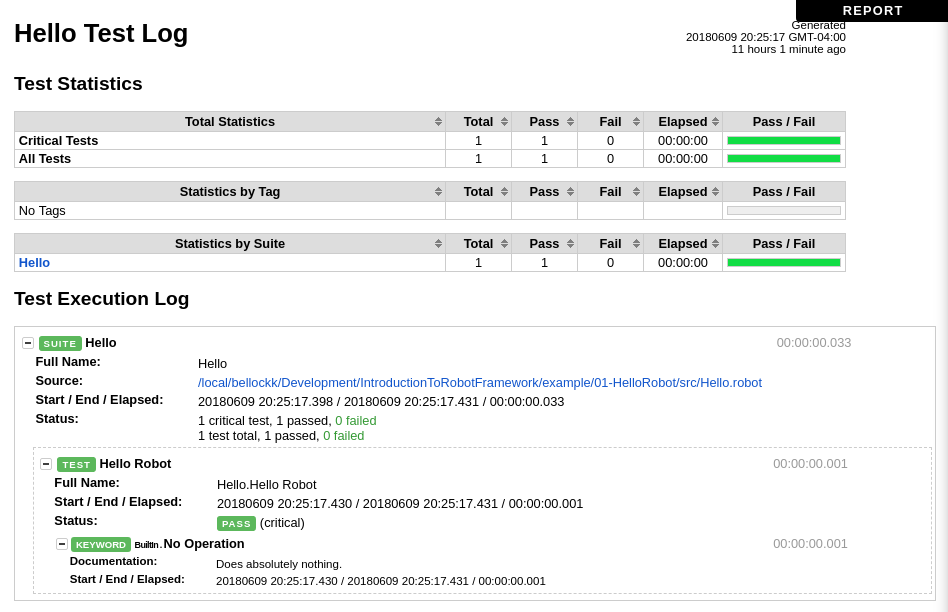
\includegraphics[width=\textwidth,height=.8\textheight,keepaspectratio]{01-log}
    \end{center}
\end{frame}

\begin{frame}\frametitle{Report}
    \begin{center}
        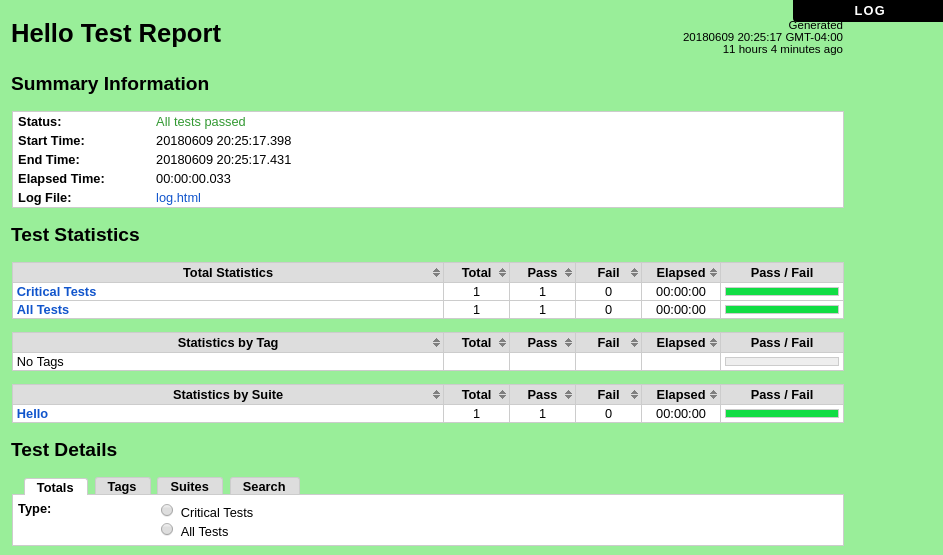
\includegraphics[width=\textwidth,height=.8\textheight,keepaspectratio]{01-report}
    \end{center}
\end{frame}

\begin{frame}\frametitle{Summary}
    \begin{itemize}
        \item With just three lines of test script, we were able to do a meet and greet with our new robot friend
        \item Robotframework, while being asked to do nothing, has done a lot of work
            \begin{itemize}
                \item Meticulously logged each step of execution
                \item Communicated with us while working
                \item Collected statistics
                \item Rendered html templates to provide log and results summaries
            \end{itemize}
    \end{itemize}
    \begin{center}
    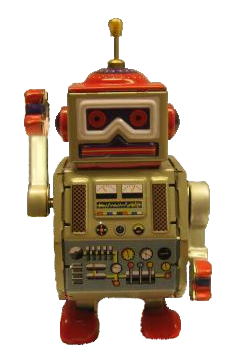
\includegraphics[height=.37\textheight]{robot-wave}
        
    \emph{And I can do so much more!}
    \end{center}
\end{frame}

\end{document}
